%!TEX root = ./main.tex
%----------------------------------------------------------------------------------------
% CASE STUDY
%----------------------------------------------------------------------------------------

\section{Case Study}\label{caseStudy} % Major section
In order to fully understand CAPA it's important to explore a case study demonstrating the process
of analysing code under test.
\lstinputlisting{./Code/CodeUnderTest.cpp}
\begin{figure}[H]
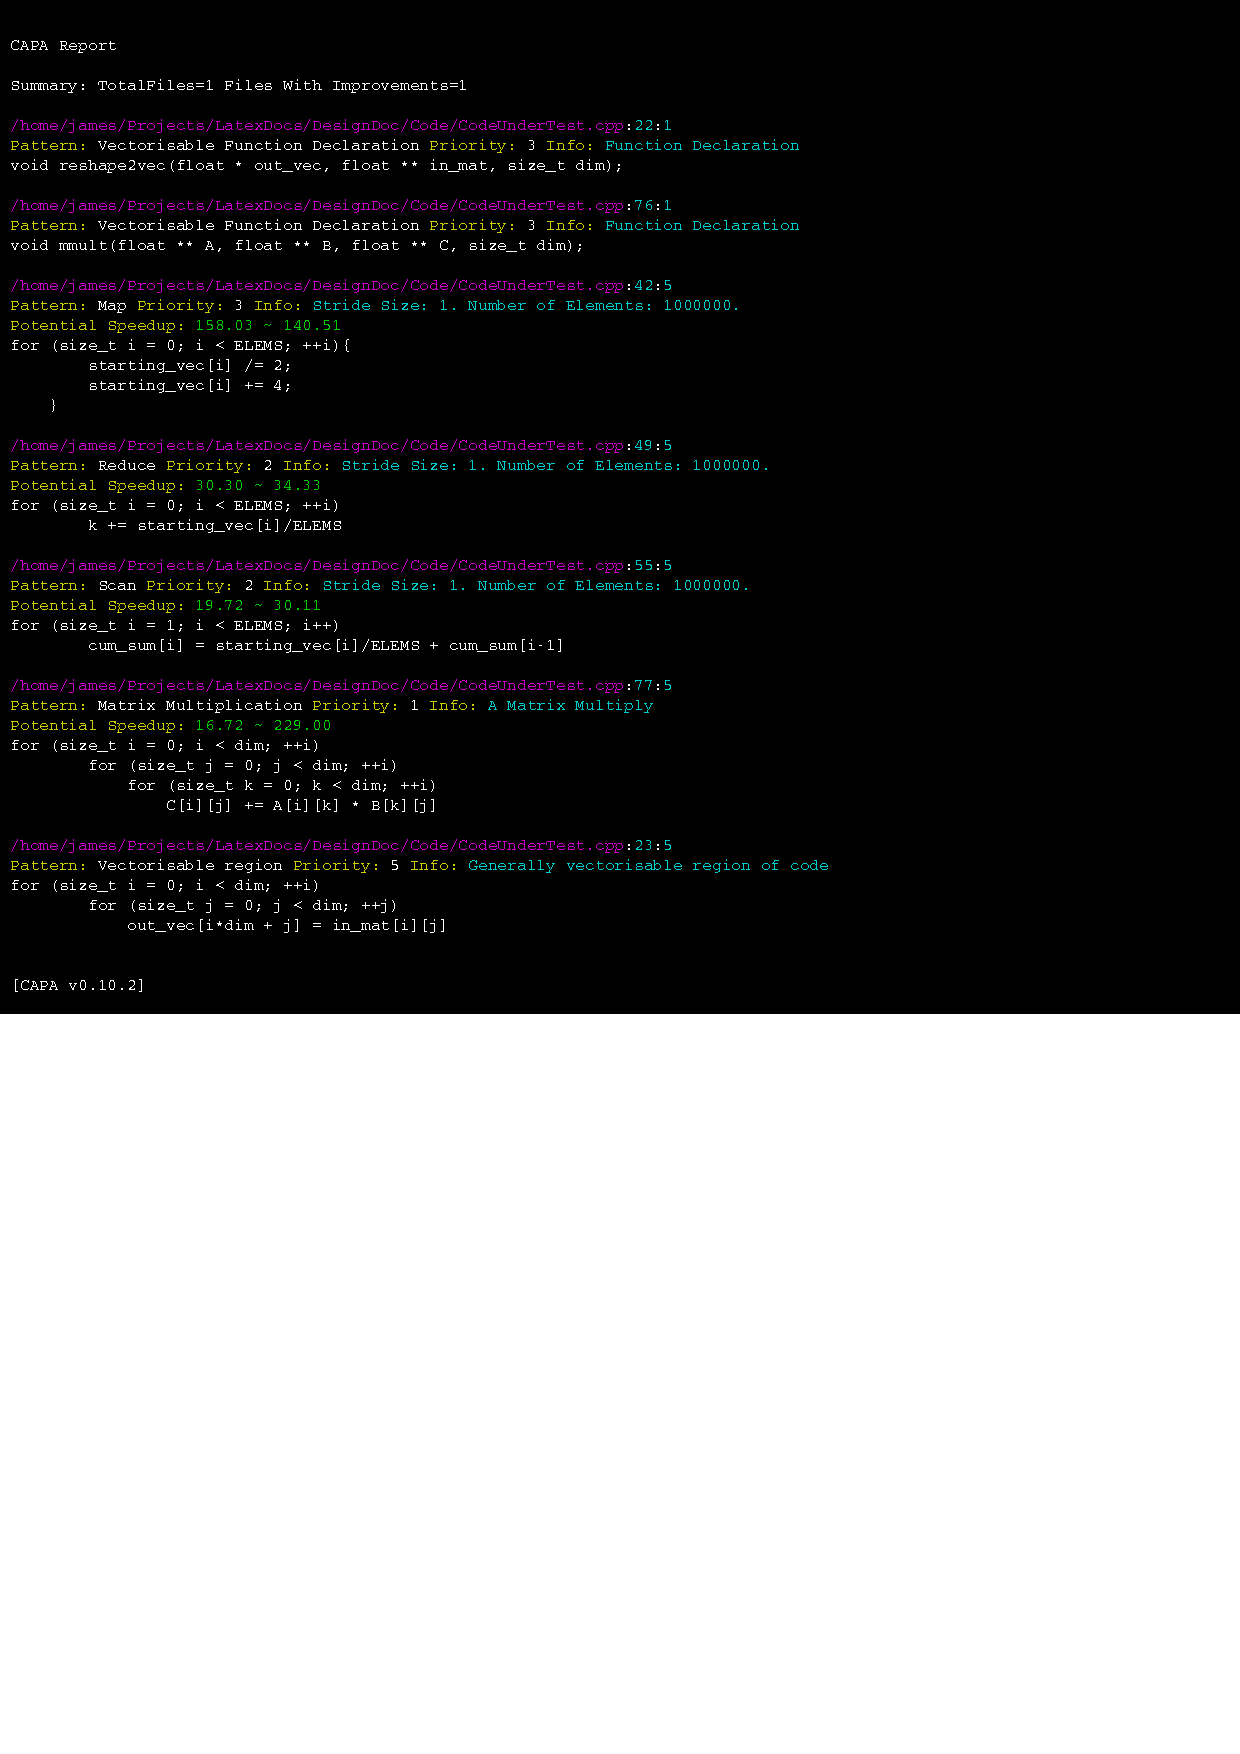
\includegraphics[clip, trim=0cm 12.7cm 6cm 0.5cm, width=\textwidth]{./Misc/report.pdf}
\caption{CAPA Generated Report}
\end{figure}
Please note that the cast study requires knowledge of the Clang AST, the output AST dump for the file
under test can be found in the Appendix at section \ref{AST}.

\subsection{Setup}
The initial setup is mostly taken care of by existing Clang and LLVM libraries. Clang Libtooling is
responsible for parsing and lexing the source file, CAPA merely passes the arguments through to the
correct Clang libraries. During the setup CAPA dynamically loads Rules for AST analysis and
Reporters for reporting. Once the rules and reporters have been loaded, CAPA loads the benchmark
information for use in the reporting phase.

Loading of rules consists of two phases. Rule Generation and Collection. Rule Generation is the
setup process whereby the AST Matchers are created, and the resulting matcher is then forwarded onto
Clang with a callback function for later processing. The rules are then collected by CAPA for
dispatching callbacks correctly.

Once the file has been loaded by the Clang front-end, parsed, and the AST constructed, the
Libtooling library begins to traverse the AST searching for a match.

\subsection{Matching}
When Clang finds a portion of the AST which matches the requirements described by the rules, the
callback function is envoked and the relevant rule must process the matching AST Node.

For our code under test, the first callback that occurs is not shown in the report, this is due to
the tag which tells CAPA to ignore that function. Further information can be found here
\ref{TaggedRegion}.

\subsubsection{Match 1: Vectorisable Function Declaration}
The first match to be reported is the result of the function declaration on line 22. The pattern
identified is a \lstinline{Vectorisable Function Declaration}. This is the simplest of all the
parallel matchers. A function declaration is deemed to be potentially vectorisable based purely on
the type information available. Vectorisable functions require an arity of at least two, with one
argument being a pointer or array type, and the other argument being a \lstinline{size_t}. This is the
most speculative of the patterns identified by CAPA, as there is very little information to work
with in a function declaration, however functions that operate on vectors in C require both a
pointer to the vector, and some information about the size of the vector, thus with that limited
information we can construct a matcher.

The matcher for this rule is described by:
\lstinputlisting{./Code/Matchers/VectorFunctionDeclRule.cpp}
The grammar here is quite simple, the matcher is requesting a callback if a function declaration is
found which has a parameter that is either an array type or a pointer type, and has any parameter
which is a \lstinline{size_t}. If this is found it is to be bound by the name \lstinline{Function}
and the callback will provide the bound nodes and additional AST context.

\paragraph{Match 2: Vectorisable Function Declaration}
The second match is also a \lstinline{Vectorisable Function Declaration}. This match however is a
the result of catching a function declaration on line 76. The process by which this function is
found is no different from the prior example. Note however that the types are different, and in this
case the matcher is in fact catching types with two levels of indirection. This rule is general
enough that it is capable of catching arbitrary levels of indirection.

\subsubsection{Match 3: Map Operation}
The third match to be reported is a map operation, which is identified on line 42. The reported
information for \lstinline{Map} operations is more thorough than the information provided for
\lstinline{Vectorisable Function Declaration}, this is because more information is available to the
callback due to a stronger grammar.
\lstinputlisting{./Code/Matchers/MapRule.cpp}
The Map matcher utilises the combinator library designed for this project in order to simplify the
top level expression. Our matcher is looking to identify loops which have an assignment where there
is a vector on both sides of the operator, or loops which have a compound binary operator and some
numeric literal. This describes most of the semantic restrictions a map operation enforces upon a
programmer however in order to extract performance information extra bindings are required.

The report states that there are 1 million elements to be processed, in order to extract this
information, the \lstinline{ForLoop} combinator provides a binding on the conditional which is
exposed in the callback. Similarly the number of elemts is also bound to by the \lstinline{ForLoop}
combinator with the respective node being exposed to the callback.

Upon a successful match, the callback function is called with the results structure. The results
structure contains all the bound nodes, as well as the AST Context. These tools are utilised in the
callback to filter out false positives, cases where the grammar of the matcher specification is not
strict enough to ensure only valid cases are matched. Within the callback the results are
re-organised into a simple class which defines a few basic operations. In order for a match to be
validated as truly representative of a Map operation, the results must be verified. This is done
through the \lstinline{MapInfo.isMap()} method, which confirms that the bound index's of the input
and ouput vectors are related without a data dependency.

Beyond validating matches, the callback is responsible for retrieving and providing information to
the reporters about the known quantities of the region. That is to say that the callback is
responsible for retrieving whatever information is available from the now exposed bound nodes.  In
order to calculate the number of elements to be processed, the right hand side of the loop condition
is constant folded to an integer. If this is possible and there is a result, that information is
then used as the number of elements to process. Similarly the stride size in the report is 1. This
is also bound by the \lstinline{ForLoop} combinator, which binds to the loop increment. This binding
is then matched against typical loop increment expressions, and where possible constant folding
extracts the stride size.

This information is then passed along to the reporter in order to provide performance metrics.

\subsubsection{Match 4: Reduce Operation}
The fourth match to be reported is a reduction, which occurs on line 49. Like the Map report, the
reduction provides more information about potential improvements. The reduction in the code under
test is the calculating of a mean, by summing the contents of the \lstinline{starting_vec} divided
by the number of elements. This is cleary a many to one operation which satisfies the requirements
of parallel reductions. 
\lstinputlisting{./Code/Matchers/ReduceRule.cpp}
In this case the matcher constructed to capture the reductino is different from the map operation,
again however it reads like english. The matcher is looking for a loop which in the body has either
an assignment or compound assignment operator, with a single value on the left, and a vector on the
right. Once this is matched, Clang passes the relevant information back via the callback which
proceeds to validate whether the region of the AST is a viable for parallelisation.

\subsubsection{Match 5: Scan Operation}
The fifth match reported is a scan operation, which occurs on line 55 of the source file. Again like
the map and reduction reports, the scan report also provides information about the number of
elements and stride size where available. The matcher is described by:
\lstinputlisting{./Code/Matchers/ScanRule.cpp}

\subsubsection{Match 6: Matrix Multiplication}
The sixth match reported is the matrix multiplication that occurs on line 77. Matrix multiplication
is not one of the parallel primitives, however it exhibits massive speed improvements when processed
on a GPU compared to a CPU. The matcher for the matrix multiplication is described by:
\lstinputlisting{./Code/Matchers/MatrixMultRule.cpp}
This matcher is slightly different from the previous examples, as it requires the nesting of
multiple loops. It still reads like plain english however. The matcher is looking for a for loop
which has a child that is a forloop which has a child that is also a forloop that has a compound
addition assignment within the body, on the left hand side of the compound assignment there is a
Matrix, which is defined as a double indexed vector, and on the right hand side there is a scalar
multiplication of two matrix elements. Referring to the AST breakdown in figure \ref{mmul_ast}, we
can see directly how the tree is matched.
\begin{figure}[H]
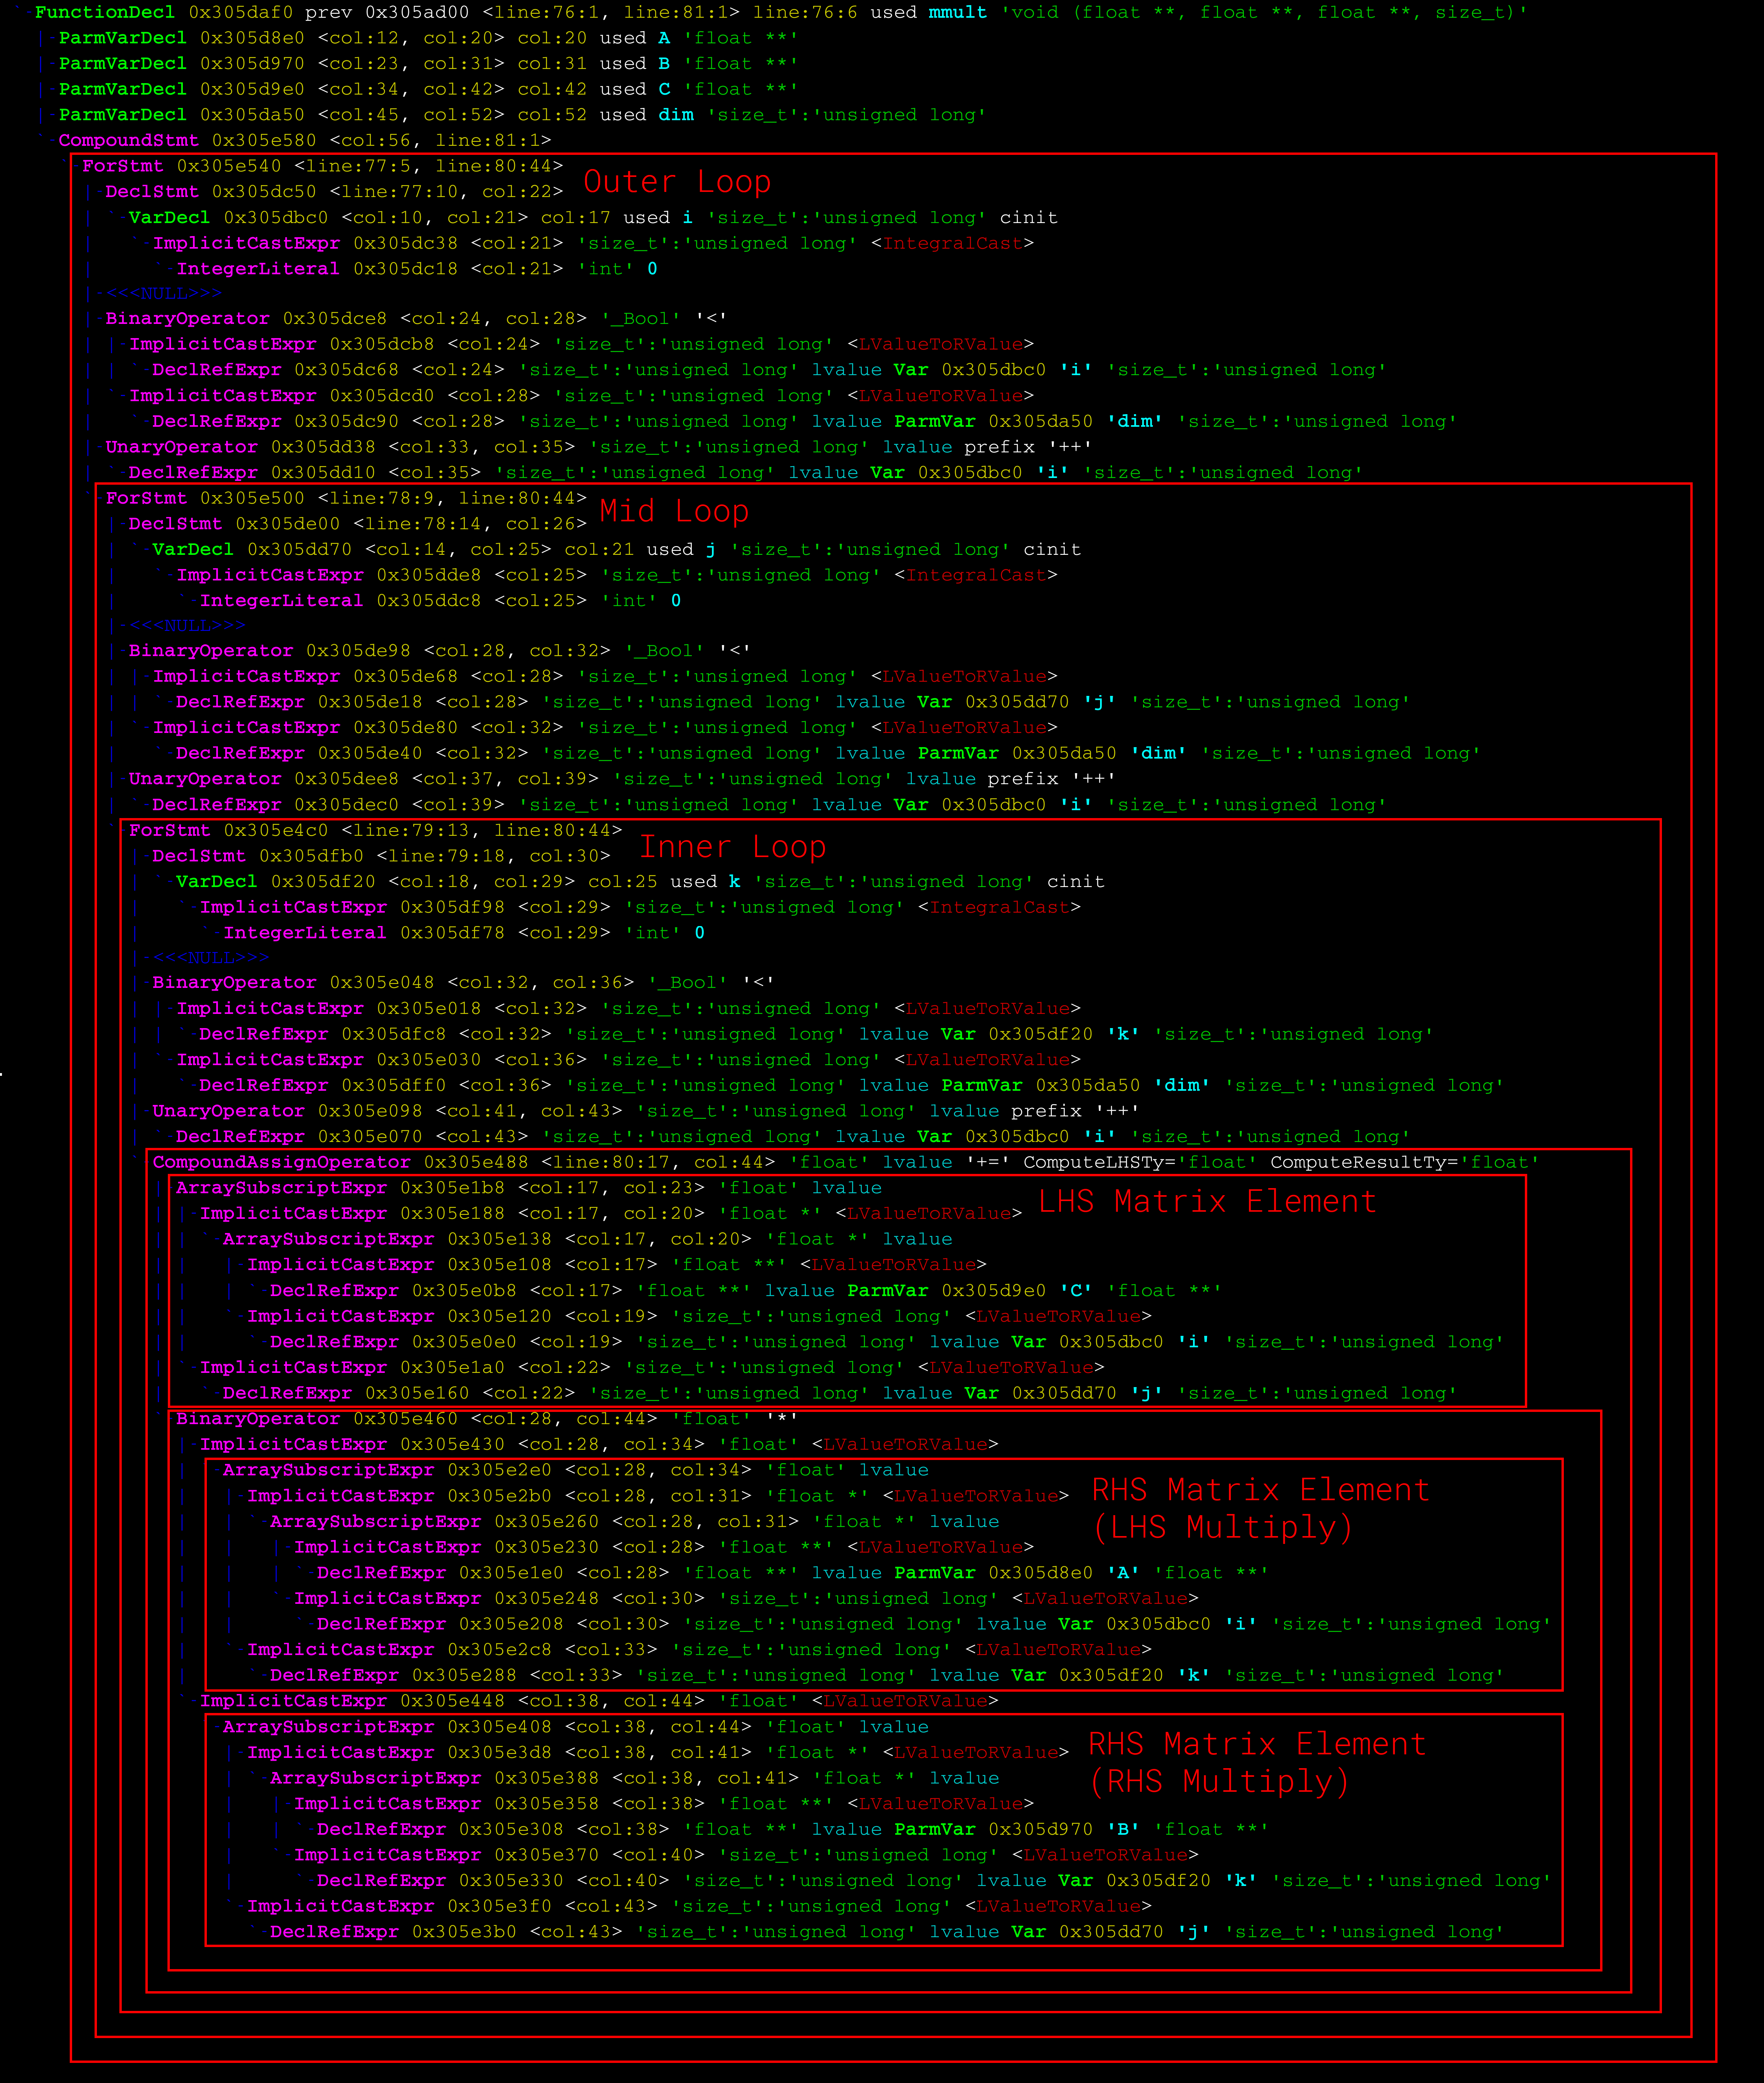
\includegraphics[width=\textwidth]{./Pictures/mmult_ast.png}
\caption{Matrix Multiplication AST Match Breakdown}\label{mmul_ast}
\end{figure}
\pagebreak

\subsubsection{Match 7: Vectorisable Region}
The seventh match reported is a generally vectorisable region has been detected. This pattern is the
most general of those reported by CAPA. The AST is queried for regions that are considered generally
vectorisable, which are then rejected if they are already tagged as a more specific operation. The
matcher for this pattern is:
\lstinputlisting{./Code/Matchers/VectorisableRule.cpp}
This matcher simply looks for a loop of any type which contains no control flow within it.
Additionally the matcher requires that any ancestor loops also not contain control flow in order to
minimise the risk of a data dependency. The operation on line 23 can not be described by any of our
GPU primitives, yet it still meets the requirements for code to be potentially parallelised. Note
however in this scenario it would be unwise to parallelise this code, as it is merely memory
operations with very minimal computational work per element.

\subsection{Tagged Regions}\label{TaggedRegion}
Within the source code there are regions marked \lstinline{///CAPA:IGNORE} and
\lstinline{/** CAPA:IGNORE */} these alert CAPA that the region is not to be reported on. CAPA
achieves this through Clang providing the structured comments interface via declaration statements.
The AST Context preserves special comments indicated by the triple slash or double asterisk,
allowing CAPA to hook into the context and retrieve comments assigned to declarations. This is
achieved via the following:
\lstinputlisting{./Code/ignore.h}
This is called from within the callback of the matchers to determine whether the region should be
processed further, or aborted. The callback is expected to pass the nearest parent declaration to
the function in order to determine whether the region should be ignored or not. The current
implementation ignores at the function declaration level.

Within the code under test there are three declarations which are marked to ignore. If we extract
those segments and remove the ignore directive, CAPA includes them in the report, resulting in this
summary:
\begin{figure}[H]
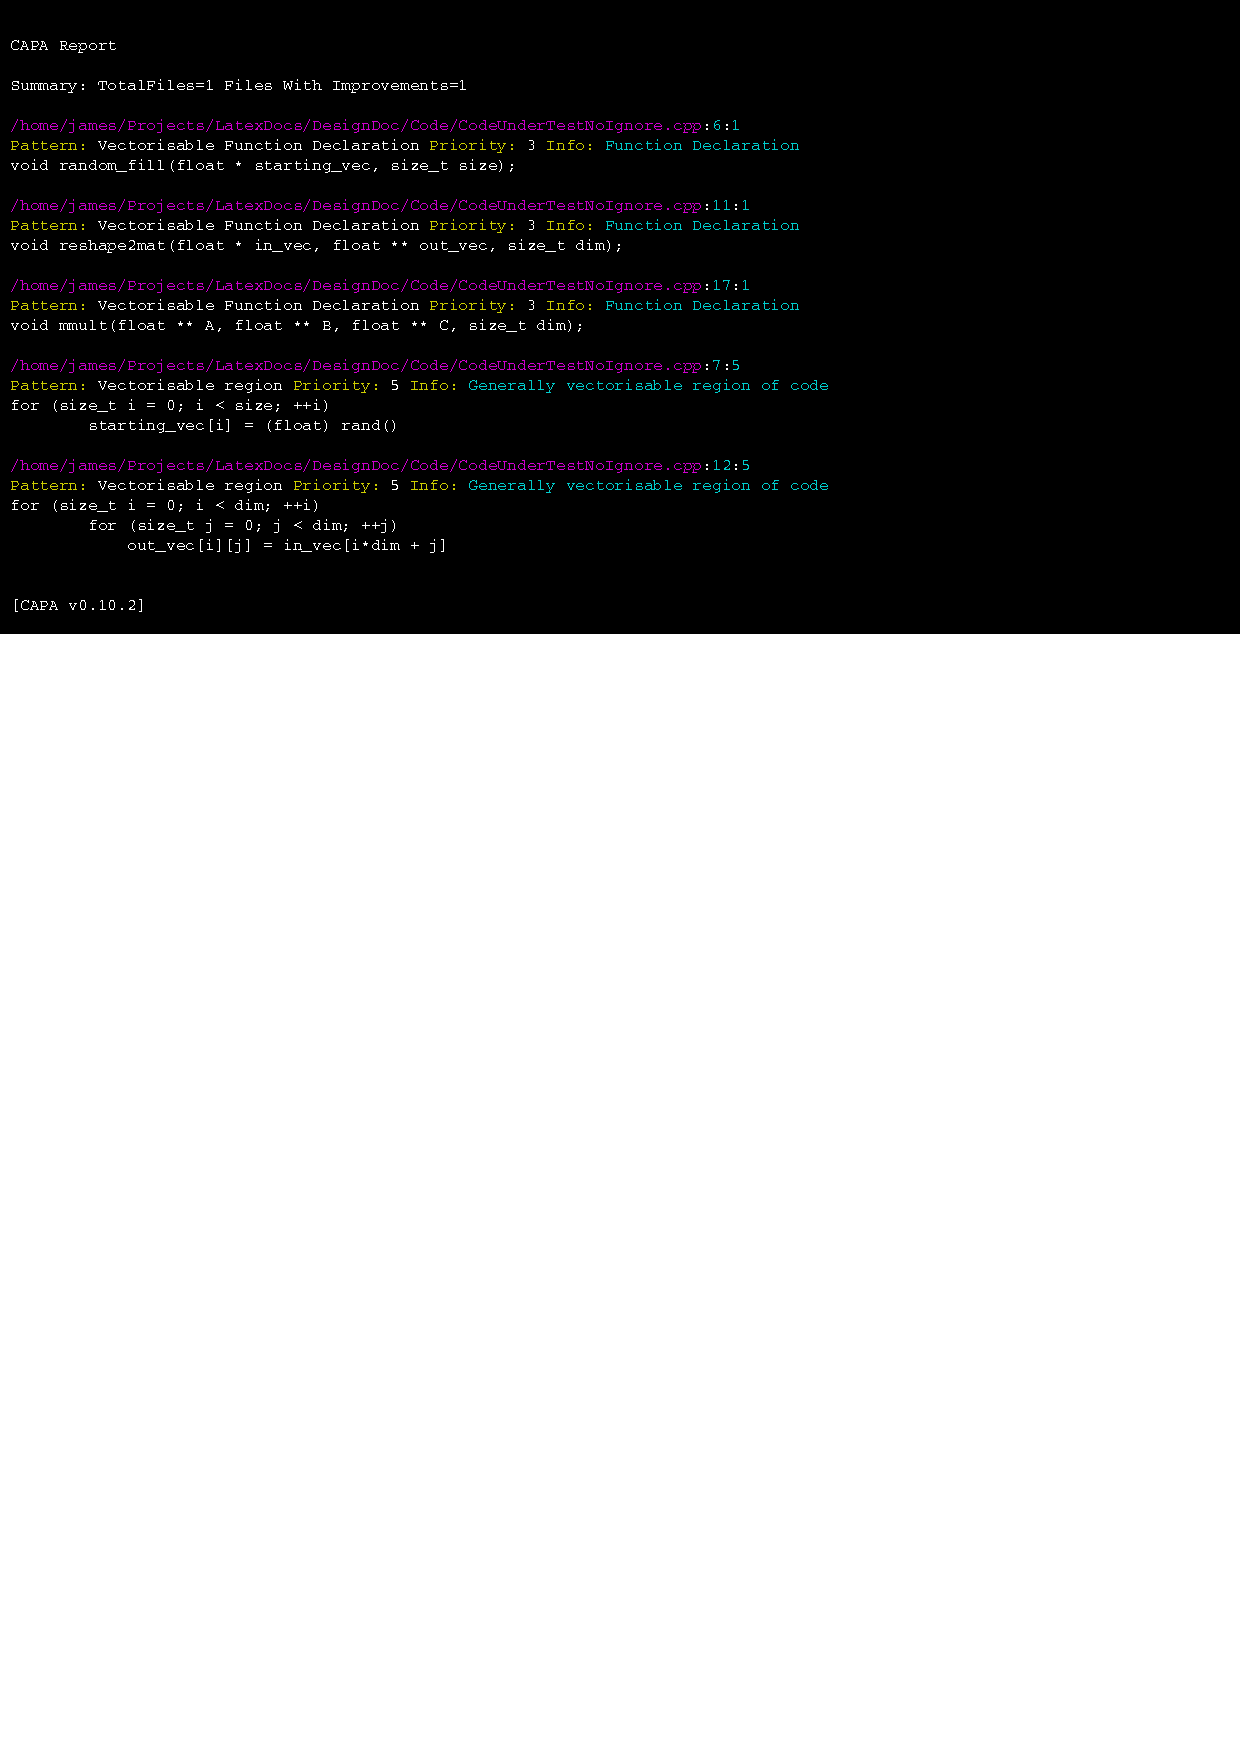
\includegraphics[clip,trim=0cm 19cm 4cm 0.5cm,width=\textwidth]{./Misc/removedIgnore.pdf}
\caption{Report without ignored regions}
\end{figure}
which now includes the previously ignored function declarations, and the vectorisable regions within
them.

\subsection{Report Generation}
The report generation is the final part of the CAPA analysis. All patterns have been identified and
filtered, the reporter is merely responsible for disaplying the information. Currently there is only
a text reporter which produces coloured output for ANSI terminals. The reporter module interfaces
with the pattern information provided by the rule set in order to report information that has been
gathered by the rules. This information is then used by the reporter to interface with the benchmark
information to produce performance characteristics which are displayed if available. In cases where
performance metrics are not available, no information is displayed.
%------------------------------------------------



